%  A simple AAU report template.
%  2013-03-06 v. 1.0.0
%  Copyright 2010-2013 by Jesper Kjær Nielsen <jkn@es.aau.dk>
%
%  This is free software: you can redistribute it and/or modify
%  it under the terms of the GNU General Public License as published by
%  the Free Software Foundation, either version 3 of the License, or
%  (at your option) any later version.
%
%  This is distributed in the hope that it will be useful,
%  but WITHOUT ANY WARRANTY; without even the implied warranty of
%  MERCHANTABILITY or FITNESS FOR A PARTICULAR PURPOSE.  See the
%  GNU General Public License for more details.
%
%  You can find the GNU General Public License at <http://www.gnu.org/licenses/>.
%
%  A simple AAU report template.
%  2015-05-08 v. 1.2.0
%  Copyright 2010-2015 by Jesper Kjær Nielsen <jkn@es.aau.dk>
%
%  This is free software: you can redistribute it and/or modify
%  it under the terms of the GNU General Public License as published by
%  the Free Software Foundation, either version 3 of the License, or
%  (at your option) any later version.
%
%  This is distributed in the hope that it will be useful,
%  but WITHOUT ANY WARRANTY; without even the implied warranty of
%  MERCHANTABILITY or FITNESS FOR A PARTICULAR PURPOSE.  See the
%  GNU General Public License for more details.
%
%  You can find the GNU General Public License at <http://www.gnu.org/licenses/>.
%
\documentclass[11pt,oneside,a4paper,openright]{report}
%\documentclass[conference]{IEEEtran}
%%%%%%%%%%%%%%%%%%%%%%%%%%%%%%%%%%%%%%%%%%%%%%%%
% Language, Encoding and Fonts
% http://en.wikibooks.org/wiki/LaTeX/Internationalization
%%%%%%%%%%%%%%%%%%%%%%%%%%%%%%%%%%%%%%%%%%%%%%%%
% Select encoding of your inputs. Depends on
% your operating system and its default input
% encoding. Typically, you should use
%   Linux  : utf8 (most modern Linux distributions)
%            latin1 
%   Windows: ansinew
%            latin1 (works in most cases)
%   Mac    : applemac
% Notice that you can manually change the input
% encoding of your files by selecting "save as"
% an select the desired input encoding. 
\usepackage[utf8]{inputenc}
 \usepackage{graphicx}
 \graphicspath{ {/home/user/Pictures/} }
% Make latex understand and use the typographic
% rules of the language used in the document.
\usepackage[danish,english]{babel}
% Use the palatino font
\usepackage[sc]{mathpazo}
\linespread{1.05}         % Palatino needs more leading (space between lines)
% Choose the font encoding
\usepackage[T1]{fontenc}
%%%%%%%%%%%%%%%%%%%%%%%%%%%%%%%%%%%%%%%%%%%%%%%%
% Graphics and Tables
% http://en.wikibooks.org/wiki/LaTeX/Importing_Graphics
% http://en.wikibooks.org/wiki/LaTeX/Tables
% http://en.wikibooks.org/wiki/LaTeX/Colors
%%%%%%%%%%%%%%%%%%%%%%%%%%%%%%%%%%%%%%%%%%%%%%%%
% load a colour package
\usepackage{xcolor}
\definecolor{aaublue}{RGB}{33,26,82}% dark blue
% The standard graphics inclusion package
\usepackage{graphicx}
% Set up how figure and table captions are displayed
\usepackage{caption}
\usepackage{subcaption}
\captionsetup{%
  font=footnotesize,% set font size to footnotesize
  labelfont=bf % bold label (e.g., Figure 3.2) font
}
% Make the standard latex tables look so much better
\usepackage{array,booktabs}
% Enable the use of frames around, e.g., theorems
% The framed package is used in the example environment
\usepackage{framed}

%%%%%%%%%%%%%%%%%%%%%%%%%%%%%%%%%%%%%%%%%%%%%%%%
% Mathematics
% http://en.wikibooks.org/wiki/LaTeX/Mathematics
%%%%%%%%%%%%%%%%%%%%%%%%%%%%%%%%%%%%%%%%%%%%%%%%
% Defines new environments such as equation,
% align and split 
\usepackage{amsmath}
% Adds new math symbols
\usepackage{amssymb}
% Use theorems in your document
% The ntheorem package is also used for the example environment
% When using thmmarks, amsmath must be an option as well. Otherwise \eqref doesn't work anymore.
\usepackage[framed,amsmath,thmmarks]{ntheorem}

%%%%%%%%%%%%%%%%%%%%%%%%%%%%%%%%%%%%%%%%%%%%%%%%
% Page Layout
% http://en.wikibooks.org/wiki/LaTeX/Page_Layout
%%%%%%%%%%%%%%%%%%%%%%%%%%%%%%%%%%%%%%%%%%%%%%%%
% Change margins, papersize, etc of the document
\usepackage[
  inner=28mm,% left margin on an odd page
  outer=41mm,% right margin on an odd page
  ]{geometry}
% Modify how \chapter, \section, etc. look
% The titlesec package is very configureable
\usepackage{titlesec}
\titleformat{\chapter}[display]{\normalfont\huge\bfseries}{\chaptertitlename\ \thechapter}{20pt}{\Huge}
\titleformat*{\section}{\normalfont\Large\bfseries}
\titleformat*{\subsection}{\normalfont\large\bfseries}
\titleformat*{\subsubsection}{\normalfont\normalsize\bfseries}
%\titleformat*{\paragraph}{\normalfont\normalsize\bfseries}
%\titleformat*{\subparagraph}{\normalfont\normalsize\bfseries}

% Clear empty pages between chapters
\let\origdoublepage\cleardoublepage
\newcommand{\clearemptydoublepage}{%
  \clearpage
  {\pagestyle{empty}\origdoublepage}%
}
\let\cleardoublepage\clearemptydoublepage

% Change the headers and footers
\usepackage{fancyhdr}
\pagestyle{fancy}
\fancyhf{} %delete everything
\renewcommand{\headrulewidth}{0pt} %remove the horizontal line in the header
\fancyhead[RE]{\small\nouppercase\leftmark} %even page - chapter title
\fancyhead[LO]{\small\nouppercase\rightmark} %uneven page - section title
\fancyhead[LE,RO]{\thepage} %page number on all pages
% Do not stretch the content of a page. Instead,
% insert white space at the bottom of the page
\raggedbottom
% Enable arithmetics with length. Useful when
% typesetting the layout.
\usepackage{calc}

%%%%%%%%%%%%%%%%%%%%%%%%%%%%%%%%%%%%%%%%%%%%%%%%
% Bibliography
% http://en.wikibooks.org/wiki/LaTeX/Bibliography_Management
%%%%%%%%%%%%%%%%%%%%%%%%%%%%%%%%%%%%%%%%%%%%%%%%
\usepackage[backend=bibtex,
  bibencoding=utf8
  ]{biblatex}
\addbibresource{bib/mybib}
\usepackage[utf8]{inputenc}

%%%%%%%%%%%%%%%%%%%%%%%%%%%%%%%%%%%%%%%%%%%%%%%%
% Misc
%%%%%%%%%%%%%%%%%%%%%%%%%%%%%%%%%%%%%%%%%%%%%%%%
% Add bibliography and index to the table of
% contents
\usepackage[nottoc]{tocbibind}
% Add the command \pageref{LastPage} which refers to the
% page number of the last page
\usepackage{lastpage}
% Add todo notes in the margin of the document
\usepackage[
%  disable, %turn off todonotes
  %colorinlistoftodos, %enable a coloured square in the list of todos
  textwidth=\marginparwidth, %set the width of the todonotes
  textsize=scriptsize, %size of the text in the todonotes
  ]{todonotes}
\usepackage{array}
\usepackage{wrapfig}
\usepackage{multirow}
\usepackage{tabu}
\usepackage{tabularx}
\usepackage{blindtext}
\usepackage{enumitem}
\usepackage{gensymb}
%%%%%%%%%%%%%%%%%%%%%%%%%%%%%%%%%%%%%%%%%%%%%%%%
% Hyperlinks
% http://en.wikibooks.org/wiki/LaTeX/Hyperlinks
%%%%%%%%%%%%%%%%%%%%%%%%%%%%%%%%%%%%%%%%%%%%%%%%
% Enable hyperlinks and insert info into the pdf
% file. Hypperref should be loaded as one of the 
% last packages
\usepackage{hyperref}
\hypersetup{%
	pdfpagelabels=true,%
	plainpages=false,%
	pdfauthor={Author(s)},%
	pdftitle={Title},%
	pdfsubject={Subject},%
	bookmarksnumbered=true,%
	colorlinks=false,%
	citecolor=black,%
	filecolor=black,%
	linkcolor=black,% you should probably change this to black before printing
	urlcolor=black,%
	pdfstartview=FitH%
	
}% package inclusion and set up of the document
% see, e.g., http://en.wikibooks.org/wiki/LaTeX/Formatting#Hyphenation
% for more information on word hyphenation
\hyphenation{ex-am-ple hy-phen-a-tion short}
\hyphenation{long la-tex}
% 
%  A simple AAU report template.
%  2015-05-08 v. 1.2.0
%  Copyright 2010-2015 by Jesper Kjær Nielsen <jkn@es.aau.dk>
%
%  This is free software: you can redistribute it and/or modify
%  it under the terms of the GNU General Public License as published by
%  the Free Software Foundation, either version 3 of the License, or
%  (at your option) any later version.
%
%  This is distributed in the hope that it will be useful,
%  but WITHOUT ANY WARRANTY; without even the implied warranty of
%  MERCHANTABILITY or FITNESS FOR A PARTICULAR PURPOSE.  See the
%  GNU General Public License for more details.
%
%  You can find the GNU General Public License at <http://www.gnu.org/licenses/>.
%
%
%
% see, e.g., http://en.wikibooks.org/wiki/LaTeX/Customizing_LaTeX#New_commands
% for more information on how to create macros

%%%%%%%%%%%%%%%%%%%%%%%%%%%%%%%%%%%%%%%%%%%%%%%%
% Macros for the titlepage
%%%%%%%%%%%%%%%%%%%%%%%%%%%%%%%%%%%%%%%%%%%%%%%%
%Creates the aau titlepage
\newcommand{\aautitlepage}[3]{%
  {
    %set up various length
    \ifx\titlepageleftcolumnwidth\undefined
      \newlength{\titlepageleftcolumnwidth}
      \newlength{\titlepagerightcolumnwidth}
    \fi
    \setlength{\titlepageleftcolumnwidth}{0.5\textwidth-\tabcolsep}
    \setlength{\titlepagerightcolumnwidth}{\textwidth-2\tabcolsep-\titlepageleftcolumnwidth}
    %create title page
    \thispagestyle{empty}
    \noindent%
    \begin{tabular}{@{}ll@{}}
      \parbox{\titlepageleftcolumnwidth}{
        \iflanguage{danish}{%
          
\includegraphics[width=\titlepageleftcolumnwidth]{figures/aau_logo_da}
        }{%
          
\includegraphics[width=\titlepageleftcolumnwidth]{figures/aau_logo_en}
        }
      } &
      \parbox{\titlepagerightcolumnwidth}{\raggedleft\sf\small
        #2
      }\bigskip\\
       #1 &
      \parbox[t]{\titlepagerightcolumnwidth}{%
      \textbf{Abstract:}\bigskip\par
        \fbox{\parbox{\titlepagerightcolumnwidth-2\fboxsep-2\fboxrule}{%
          #3
        }}
      }\\
    \end{tabular}
    \vfill
    \iflanguage{danish}{%
      %\noindent{\footnotesize\emph{Rapportens indhold er frit tilgængeligt, men offentliggørelse (med kildeangivelse) må kun ske efter aftale med forfatterne.}}
    %}{%
      %\noindent{\footnotesize\emph{The content of this report is freely available, but publication (with reference) may only be pursued due to agreement with the author.}}
    }
    \clearpage
  }
}

%Create english project info
\newcommand{\englishprojectinfo}[8]{%
  \parbox[t]{\titlepageleftcolumnwidth}{
    \textbf{Title:}\\ #1\bigskip\par
    \textbf{Theme:}\\ #2\bigskip\par
    \textbf{Project Period:}\\ #3\bigskip\par
    \textbf{Project Group:}\\ #4\bigskip\par
    \textbf{Participant(s):}\\ #5\bigskip\par
    \textbf{Supervisor(s):}\\ #6\bigskip\par
    \textbf{Copies:} #7\bigskip\par
    \textbf{Page Numbers:} \pageref{LastPage}\bigskip\par
    \textbf{Date of Completion:}\\ #8
  }
}

%Create danish project info
\newcommand{\danishprojectinfo}[8]{%
  \parbox[t]{\titlepageleftcolumnwidth}{
    \textbf{Titel:}\\ #1\bigskip\par
    \textbf{Tema:}\\ #2\bigskip\par
    \textbf{Projektperiode:}\\ #3\bigskip\par
    \textbf{Projektgruppe:}\\ #4\bigskip\par
    \textbf{Deltager(e):}\\ #5\bigskip\par
    \textbf{Vejleder(e):}\\ #6\bigskip\par
    \textbf{Oplagstal:} #7\bigskip\par
    \textbf{Sidetal:} \pageref{LastPage}\bigskip\par
    \textbf{Afleveringsdato:}\\ #8
  }
}

%%%%%%%%%%%%%%%%%%%%%%%%%%%%%%%%%%%%%%%%%%%%%%%%
% An example environment
%%%%%%%%%%%%%%%%%%%%%%%%%%%%%%%%%%%%%%%%%%%%%%%%
\theoremheaderfont{\normalfont\bfseries}
\theorembodyfont{\normalfont}
\theoremstyle{break}
\def\theoremframecommand{{\color{gray!50}\vrule width 5pt \hspace{5pt}}}
\newshadedtheorem{exa}{Example}[chapter]
\newenvironment{example}[1]{%
		\begin{exa}[#1]
}{%
		\end{exa}
}% my new macros

\begin{document}
%frontmatter
\pagestyle{empty} %disable headers and footers
\pagenumbering{roman} %use roman page numbering in the frontmatter
%  A simple AAU report template.
%  2013-03-06 v. 1.0.0
%  Copyright 2010-2013 by Jesper Kjær Nielsen <jkn@es.aau.dk>
%
%  This is free software: you can redistribute it and/or modify
%  it under the terms of the GNU General Public License as published by
%  the Free Software Foundation, either version 3 of the License, or
%  (at your option) any later version.
%
%  This is distributed in the hope that it will be useful,
%  but WITHOUT ANY WARRANTY; without even the implied warranty of
%  MERCHANTABILITY or FITNESS FOR A PARTICULAR PURPOSE.  See the
%  GNU General Public License for more details.
%
%  You can find the GNU General Public License at <http://www.gnu.org/licenses/>.
%
\pdfbookmark[0]{Front page}{label:frontpage}%
\begin{titlepage}
  \addtolength{\hoffset}{0.5\evensidemargin-0.5\oddsidemargin} %set equal margins on the frontpage - remove this line if you want default margins
  \noindent%
  \begin{tabular}{@{}p{\textwidth}@{}}
    \toprule[2pt]
    \midrule
    \vspace{0.2cm}
    \begin{center}
    \Huge{\textbf{
      Turtlesim % insert your title here
    }}
    \end{center}
    \begin{center}
      \Large{
        - The mover -% insert your subtitle here
      }
    \end{center}
    \vspace{0.2cm}\\
    \midrule
       
    \toprule[2pt]
  \end{tabular}
    \begin{figure}[h]
    \begin{center}
    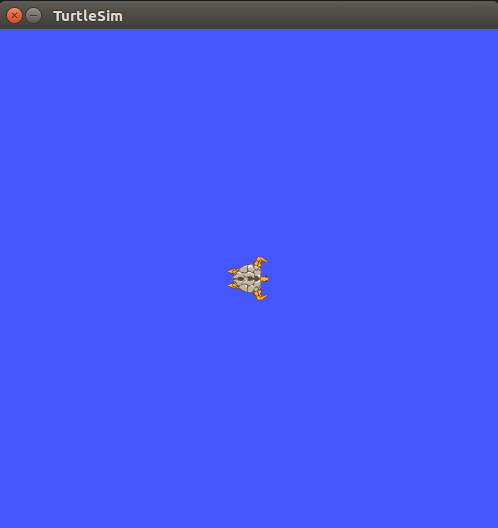
\includegraphics[width=.5\textwidth]{figures/turtlesim.png}
     \end{center}
    \end{figure}
    
  \vspace{2 cm}
  \begin{center}
    {\large
      Project Report%Insert document type (e.g., Project Report)
    }\\
    \vspace{0.2cm}
    {\Large
      B2-19\\
      Mini-projcet\\
      Programming
      %Insert your group name or real names here
    }
  \end{center}
  \vfill
 \end{titlepage}
\clearpage

\cleardoublepage
\pdfbookmark[0]{Contents}{label:contents}
\pagestyle{fancy} %enable headers and footers again
\tableofcontents
\chapter*{Preface\markboth{Preface}{Preface}}\label{ch:preface}
\addcontentsline{toc}{chapter}{Preface}


\vspace{\baselineskip}\hfill Aalborg University, \today
\vfill\noindent
\begin{minipage}[b]{0.45\textwidth}
 \centering
 \rule{\textwidth}{0.5pt}\\
  Valdemar Jul Qvist\\
 {\footnotesize <vqvist17@student.auu.dk>}
\end{minipage}
\hfill
\begin{minipage}[b]{0.45\textwidth}
 \centering
 \rule{\textwidth}{0.5pt}\\
  Mark Richard Blankensteiner\\
 {\footnotesize <mblank16@student.aau.dk>}
\end{minipage}
\vspace{3\baselineskip}
\begin{center}
\begin{minipage}[b]{0.45\textwidth}
 \centering
 \rule{\textwidth}{0.5pt}
  Anders Fischer Steen Jensen\\
 {\footnotesize <afsj16@student.aau.dk>}\\
 \vspace{2 cm}
\end{minipage}
\end{center}
\begin{minipage}[b]{0.45\textwidth}
 \centering
 \rule{\textwidth}{0.5pt}\\
  Violeta Kuldaite\\
 {\footnotesize <vkulda17@student.aau.dk>}
\end{minipage}
\hfill
\begin{minipage}[b]{0.45\textwidth}
 \centering
 \rule{\textwidth}{0.5pt}\\
  Natalie Mark\\
 {\footnotesize <nmark15@student.aau.dk>}
\end{minipage}

\cleardoublepage
%mainmatter
\pagenumbering{arabic} %use arabic page numbering in the mainmatter
\chapter{Introduction}\label{ch:introduction}

In this chapter the there will be introduce the workings off the 2 nodes.

\section{UI\_Turtlesim\_mover node}

The UI\_Turtlesim\_mover node, is the publisher to the Turtlesim\_mover node.\\
This program will ask whether you want the Turtlesim to draw a circle, square or star. Hereby the user can press 1,2,3 accordingly to what type of object the user want drawn. This will then send a topic to the subscriber, with information about the choice which the user made.\\


\section{Turtlesim\_mover node}


The Turtlesim\_mover node is the node that makes the turtlesim move in a square, circle or random moving.\\
It listens to the topic that the UI publishes on, when the user picks a choice for the turtlesim.
It will send a messages back to the UI node and confirm that it needs some thing to do or it is doing the command of the user.\\
\chapter{A look into the codes} \label{ch:lookinto}

In this chapter segments of the code will be explained.

\section{Include files} 

The compiler will always look through the code in a linear fashion, which is why it is required to include all the files that is necessary in the code, in the first lines of code.\\

\begin{figure}[h]
\begin{center}
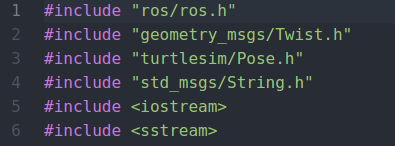
\includegraphics[width=.5\textwidth]{figures/therealinclude.png}
\caption{Include files}
\end{center}
\end{figure}\label{fig:include}

\begin{itemize}
\item \texttt{ros/ros.h}\\
This is a header to include all the headers necessary for the commonly used pieces in the ROS system.\\
\item \texttt{geometry\_msgs/Twist.h}\\
Includes the headers for the commonly used geometrics, like poses, vectors and points.\\
\item \texttt{turtlesim/pose.h}\\
This header file is only needed in the \texttt{Turtlesim\_mover}, since turtlesim/pose is a publisher.\\
This creates the headers for the pose of the virtual turtle.\\
\item \texttt{std\_msgs/String.h}\\
Is an automatized string header, which is generated from the String.msg file.\\
\item \texttt{<iostream>}\\
This is the input/output stream and helps with just that.\\
\item \texttt{<sstream>}\\
Includes the std::stringstream.\\

\end{itemize}


\section{The node handler}
Before it is possible to use any ROS components there must be a initiation of ROS see first line in figure \ref{fig:nodehandel}. The init needs 3 arguments argv, argc and a name. In this one it is called publish\_velocity. The nodehandle in figure \ref{fig:nodehandel} on the second line, is needed to initiate the node. The nodehandle is declared to be "n" in the mover node.
\begin{figure}[h]
\begin{center}
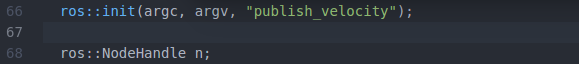
\includegraphics[width=.9\textwidth]{figures/nodehandel.png}
\caption{initiation of node-handle}
\end{center}
\end{figure}\label{fig:nodehandel}


\section{Publisher}
\begin{figure}[h]
\begin{center}
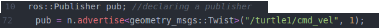
\includegraphics[width=.9\textwidth]{figures/publisher.png}
\caption{Publisher}
\end{center}
\end{figure}\label{fig:publihser}
The publisher need to be declared as a variable, which is done on the first line see figure \ref{fig:publihser}.The next line show the message which is published, in this case a geometry::Twist and what topic it is published on /turtle1/cmd\_vel.


\section{Subscriber}
The subscriber has more or less the same syntax to be declared as a publisher see figure \ref{fig:subscriber}. The syntax is a bit different, in the way, that it does not need to know what message it has to listen for, but only which topic it need to subscribe to. In the case of this subscriber it listens to what is published on the Commands topic, it can put up to 1000 messages into a queue, if there are more in the buffer, they will get discarded.\\ 
To access the subscriber the function named chatterCallback is necessary, and every time something is published on the topic Commands it will be written to the chatterCallback function.

\begin{figure}[h]
\begin{center}
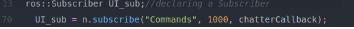
\includegraphics[width=.9\textwidth]{figures/subscriber.png}
\caption{subscriber}
\end{center}
\end{figure}\label{fig:subscriber}

\section{UI\_turtlesim\_mover}

Firstly the include files are introduced.\\
Afterwards the global parameters are set, such as:\\
\texttt{ros::Publisher pub1;}\\
\texttt{ros::Subscriber sub1;}\\
\texttt{string done;}\\
then a void function is created.\\

\begin{figure}[h]
\begin{center}
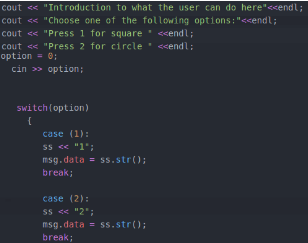
\includegraphics[width=.5\textwidth]{figures/switch.png}
\caption{VoidFunction of UI}
\end{center}
\end{figure}\label{fig:switch}

The void function as seen in figure \ref{fig:switch}, introduces a series of cout, which will print the text to the users screen.\\
Then the cin option appears. It will determine whether the user will press 1 or 2, and will then store the choice in "Option".\\
This leads to the next step in the code which is the switch. The switch, in this code, is used for the user to stay in the program. This gives the opportunity to the user to stay in the program and give multiple commands to the publisher.\\
When storing the data "1" in the cin, the switch will then use the stored data to move it through case(1). When in case(1), the code will then send the data through a message string which will "talk" to the listener. Hereby the user can acknowledge that the turtlesim will react accordingly to the user input. Lastly the code will spinOnce and return to the main function.\\
After the nodehandle, publisher, main function, init:: and subscriber is set, see figure \ref{fig:publihser}, and \ref{fig:subscriber}, it will go into a while loop.\\
\texttt{while(ros::ok())}\\
The code will now only break when the user closes the command "ctrl+c", all nodehandles has been destroyed or the nodes are pushed off the internet.\\
While ros is okay, the for loop will then run, which means that if the expression inside the loop is true, then the loop will run until the expression is false. This loop is used for making a specific code run the desired amount of times.\\
In the end it will make the loop spinOnce, and then return 0;\\

\section{Turtlesim\_mover}

In this node there is an need for having the position of the turtlesim. The method as above is used the differences is that the turtlesim publishes the position on the topic "/turtle1/pose" and the turtlesim::Pose is the message that gets published. Every time the turtlesim moves or turns a new message is published. The void function poseCallback then set the coordinates for the turtlesim in the variables xr, yr and the heading in dr. The dr has be converted from a radian to degrees that makes it easier to work with and it is multiplied 100 to get more acquired see figure \ref{fig:pose}. The data in the message is a float 64 see picture\ref{fig:turtlesimPose}, this gets converted to an integer because integers is exact not as floats that is an approximate value.\\

\begin{figure}[h]
\begin{center}
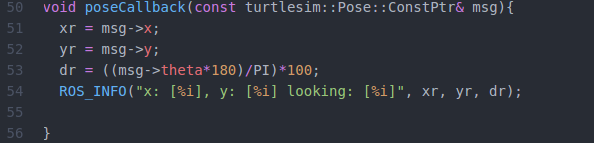
\includegraphics[width=.5\textwidth]{figures/posecall.png}
\caption{poseCallback}\label{fig:pose}
\end{center} 
\end{figure}

A subscriber is declared  that listens to the topic "Commands", on this topic is published a std::msgs message, see \ref{fig:stdmsgs}, that by the UI\_turtlesim\_mover. There is declared a void function that set a variable. When a new std::msgs messages is published on the topic "Commands", the data in the message gets stored in a string variable "ans" see figure \ref{fig:ChatterCallback}.\\
\begin{figure}[h!]
\begin{center}
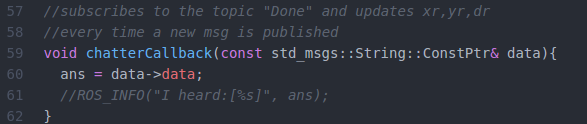
\includegraphics[width=.5\textwidth]{figures/chatterCallback.png}
\caption{ChatterCallback}\label{fig:ChatterCallback}
\end{center}
\end{figure}


The "ans" variable is set to "1" the first if statement is evaluated to true see figure \ref{fig:while}.Then the it enters the if statement and calls function named moving  that publishes to the UI\_turtlesim\_mover that the turtlesim is moving.\\

\begin{figure}[h]
\begin{center}
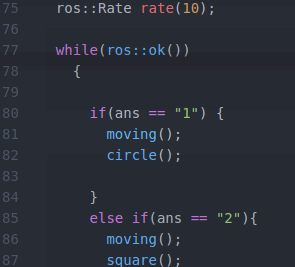
\includegraphics[width=.5\textwidth]{figures/while.png}
\caption{While loop}\label{fig:while}
\end{center}
\end{figure}

Then it calls the void function circle. In the function circle the while loop while run until statement in the brackets is not true see figure \ref{fig:while}. In the loop a linear and an angular velocity stored in the msg, that reference to the geometry\_msgs::Twist messages. The message is then publishing on the topic "/turtle1/cmd\_vel" and ros will spin once to make sure that the message is published.\\  When the dr is above 35900 or 359${^\circ}$ the circle function will return to main function.

\begin{figure}[h]
\begin{center}
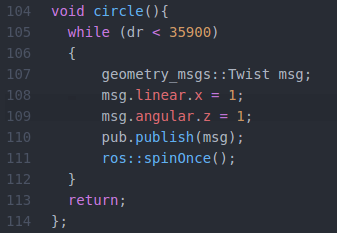
\includegraphics[width=.5\textwidth]{figures/void-circle.png}
\caption{The function circle}\label{fig:void-circle}
\end{center}
\end{figure}

\section{RandomWalk}

A simple code for randomwalk is introduced here:

\begin{figure}[h]
\begin{center}
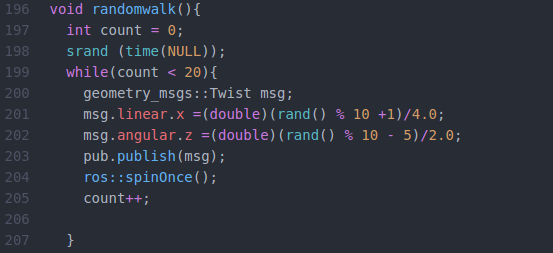
\includegraphics[width=.5\textwidth]{figures/randomWalk.png}
\caption{The function random walk}\label{fig:randomWalk}
\end{center}
\end{figure}

The code focusses on a random number. This is stated through Srand(Time(NULL)), where Srand will keep giving random steps to the turtlesim and the NULL will keep making the numbers different from each other. This is an important process for the RandomWalk since it must not repeat itself.\\
So the code is given a loop to repeat while(count>20), and count=0;. Hereby this loop will continue until the process is shut down or the count has surpassed 20.\\
The path which the message has to be sent by is geometry\_message::twist. This means that the linear and angular messages will x and z will be given integers (double) with random numbers in it, so it will move accordingly to the random number present in that loop. These random numbers has to be stated in the interval from 1-10 and 5-10, since it is forced upon the x and z in (10\%+1) and (10\%-5).\\
In the end it will SpinOnce and then the count++ will make the value rise after every execute, which will stop the process when count=20.\\
\chapter{Conclusion}\label{ch:conclusion}

%The communication between the two nodes is established by "UI\_turtlesim\_mover" and "turtlesim\_mover". These nodes talk to eachother by sending strings of information between them by topics.\\
%To conclude, the code has met the standards which was set from the start. \\
%The code will execute the commands send in by the user and show exactly how it works by demonstrating the message in turtlesim.

The aim for this mini-project has been to focus on communication of the nodes and what they publish.\\ In the process of building the nodes, for manipulating the turtlesim, gave a clear understanding of the interactions between nodes in the ROS system.\\
The nodes was build in a way that the user-interface, would have control over what needed to be published. By using the \texttt{topic list} we could clearly see what topics was used in the turtlesim, when we listened to these topics while moving the turtle it was possible to determine what data was published. We could determine that the turtlesim\_mover needed to send a string of commands to the turtlesim. While the listener was connected to turtlesim, it would then process the message and visualize what has been written in the terminal will affect a third-party program.\\

%\bibliographystyle{unsrt}
%\bibliography{bib/mybib.bib}
\printbibliography[heading=bibintoc]
\label{bib:mybiblio}
\appendix
\chapter{Appendix A}\label{ch:appAlabel}
\section{msgs types}
\begin{figure}[h]
\centering
    \begin{subfigure}{.49\textwidth}
        \centering
        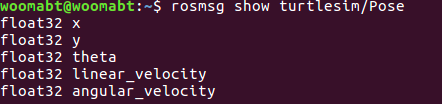
\includegraphics[width=\textwidth]{figures/turtlesim_pose.png}
        \caption{turtlesim\_pose}
        \label{fig:turtlesimPose} 
    \end{subfigure}
    \begin{subfigure}{.49\textwidth}
        \centering
        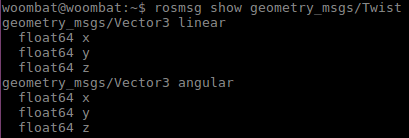
\includegraphics[width=\textwidth]{figures/geometry_msg.png} 
        \caption{geometry\_msgs/Twist}
        \label{fig:geometry\_msg\_Twist}
    \end{subfigure}
\caption{what is inside msgs}
\label{fig:whatisinside}
\end{figure}
\begin{figure}[h]
    \begin{center}
    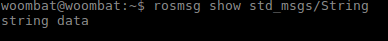
\includegraphics[width=.55\textwidth]{figures/stdmsgs.png}
    \caption{Std\_msgs/string}
    \label{fig:stdmsgs}
    \end{center}
\end{figure}
\chapter{Appendix B source code}\label{ch:appBlabel}


\begin{itemize}
    
    
    \item The source code is included in a tar.gz
    \item The source code is also available on git hub:\\https://github.com/ValdemarQvist/b2-19-talker.git\\
    \item Demo of the node working together on three computers



\end{itemize}




\end{document}
